\subsection{Linear-Probe Analysis of Cue-Conditioned Representations}
\label{app:coin-city-mechanistic-probe}

\subsubsection{Behavioral Screening Criteria}
We screen the same held-out prompts with Qwen3-8B, Qwen3-14B, dense Qwen3-32B, and
Qwen2.5-72B-Instruct. Each checkpoint received 16 test episodes crossed with
$k\in\{0,4\}$ and correct, absent, or inverted City C context (96 prompts), with
96/96 parseable forecasts.

\begin{center}
\begin{minipage}{\linewidth}
\centering
\captionof{table}{\textbf{Behavioral screening results for the linear-probe analysis.}
Entries are paired mean differences with 95\% episode-bootstrap intervals
($n=16$). Evidence is no-context $k=4$ minus $k=0$ aligned slope; selection is
correct minus absent context at $k=0$; reversal is inverted minus correct context
at $k=0$; forecast penalty is inverted minus correct poll MAE at $k=0$. Positive
evidence and selection, negative reversal, and a positive forecast penalty are
the predicted directions.}
\label{tab:coin-city-behavioral-gate}
\scriptsize
\setlength{\tabcolsep}{2.4pt}
\resizebox{\linewidth}{!}{% Generated by paper/generate_coin_city_mechanistic_comparison.py; do not edit.
\begin{tabular}{lcccc}
\toprule
Model & Evidence & Selection & Reversal & Forecast penalty \\
\midrule
Qwen3-8B & $+.119$ $[-.094,+.374]$ & $+.078$ $[-.012,+.219]$ & $-.140$ $[-.315,+.007]$ & $+.812$ $[-.063,+2.023]$ \\
Qwen3-14B & $+.394$ $[+.152,+.734]$ & $+.261$ $[+.134,+.400]$ & $-.380$ $[-.597,-.172]$ & $+1.662$ $[+.252,+3.155]$ \\
Qwen3-32B & $+.315$ $[+.017,+.646]$ & $+.234$ $[+.111,+.407]$ & $-.390$ $[-.554,-.221]$ & $+1.965$ $[+1.013,+3.083]$ \\
Qwen2.5-72B & $+.246$ $[+.001,+.529]$ & $+.096$ $[-.077,+.259]$ & $-.433$ $[-.674,-.220]$ & $+2.206$ $[+.957,+3.620]$ \\
\bottomrule
\end{tabular}
}
\end{minipage}
\end{center}

The 14B and 32B intervals exclude zero in all four predicted directions. For 72B,
the evidence, reversal, and forecast-penalty intervals exclude zero, while the
correct-versus-absent selection interval spans zero. All four 8B intervals span
zero. We use 32B for the dense Qwen3 scaling comparison and 72B for a
cross-generation comparison; neither is interpreted as another point on a
monotonic size curve. Qwen3-4B and Llama-3.1-8B use the identical task file,
held-out split, and model, layer, target, and endpoint selection rules.

\subsubsection{Activation and Probe Protocol}
We selected 64 episodes without replacement, balanced over which reference city
was strongly responsive and whether City C's latent regime was strong or weak.
Forty-eight episodes form a development set and 16 form a sealed test set. Each
episode is rendered at $k=0$ and $k=4$ under correct, absent, and inverted context,
giving 384 activation records. Within an episode-prefix pair the three prompts
have identical numeric content. The only intervention is the City C relationship
description.

For the final input token, we save the embedding output and every transformer-block
output. The resulting tensor dimensions are $[384,37,2560]$ for Qwen3-4B;
$[384,37,4096]$ for Qwen3-8B; $[384,33,4096]$ for Llama-3.1-8B;
$[384,41,5120]$ for Qwen3-14B; $[384,65,5120]$ for Qwen3-32B; and
$[384,81,8192]$ for Qwen2.5-72B-Instruct. We fit separate dual-ridge probes at
each layer and $k$, using only correct-context development episodes. Four
cell-balanced development folds select the ridge strength from
$\{10^{-4},3\!\times\!10^{-3},10^{-1},3,100\}$ and then select one reported
layer. The untouched test episodes are evaluated in all three context arms
($n=16$ per arm). A 10,000-repeat held-out label permutation test keeps the
development-selected layer, ridge strength, and fitted probe fixed. Thus neither
the test labels nor test-arm scores select the reported layer.

We probe three increasingly strict targets: the binary strong/weak regime; the
full realized slope $g_C$; and the within-regime residual
$g_C-.90$ for strong episodes or $g_C-.25$ for weak episodes. The first two are
recoverable from the displayed evidence and the third is not, by construction:
Section~\ref{app:coin-city-probe-ceilings} derives what a Bayes-optimal reader of
the same prompt could score on each, and the residual is included as a
specificity control rather than as a target a model could hit. Mean-pooled
embedding and final-layer states are additional pooling controls.

\begin{center}
\begin{minipage}{\linewidth}
\centering
\captionof{table}{\textbf{Six-model correct-context probe summary.}
Each entry gives $k=0/k=4$ on the 16 sealed episodes. Layers and ridge strengths
were selected on development episodes only. Residual $p$ is the one-sided
10,000-repeat held-out label-permutation value.}
\label{tab:coin-city-mechanistic-summary}
\small
\setlength{\tabcolsep}{3.0pt}
\resizebox{\linewidth}{!}{% Generated by paper/generate_coin_city_mechanistic_comparison.py; do not edit.
\begin{tabular}{lcccc}
\toprule
Model & Regime AUC & Full-slope $R^2$ & Residual-slope $R^2$ & Residual $p$ \\
\midrule
Qwen3-4B & 1.000/1.000 & .960/.885 & -.389/-.227 & .927/.614 \\
Qwen3-8B & .844/1.000 & .713/.653 & -.359/-.374 & .502/.735 \\
Llama-3.1-8B & 1.000/.984 & .913/.731 & -.126/-.207 & .380/.572 \\
Qwen3-14B & 1.000/.984 & .898/.627 & -.531/-.128 & .315/.450 \\
Qwen3-32B & 1.000/1.000 & .967/.811 & -.269/.003 & .477/.221 \\
Qwen2.5-72B & 1.000/1.000 & .975/.869 & -.451/-.053 & .675/.447 \\
\bottomrule
\end{tabular}
}
\end{minipage}
\end{center}

\begin{center}
\begin{minipage}{\linewidth}
\centering
\captionof{table}{\textbf{Held-out layer-wise open-weight probe.} AUC is reported
for the regime target and $R^2$ for both slope targets. Correct, none, and wrong
score the same development-selected probe against the true City C target under
the three context arms; wrong/cue instead scores the inverted arm against the
relationship named by its cue. $p$ is the one-sided held-out label-permutation
value on the correct-context test episodes.}
\label{tab:coin-city-mechanistic-probe}
\scriptsize
\setlength{\tabcolsep}{2.4pt}
\resizebox{\linewidth}{!}{% Generated by paper/generate_coin_city_mechanistic_comparison.py; do not edit.
\begin{tabular}{lllr rrrrrr}
\toprule
Model & $k$ & Target & Layer & Dev CV & Correct & None & Wrong/true & Wrong/cue & $p$ \\
\midrule
Qwen3-4B & 0 & Regime (AUC) & 1 & 1.000 & 1.000 & .562 & .000 & 1.000 & $<.001$ \\
 &  & Full slope ($R^2$) & 24 & .936 & .960 & -.517 & -2.614 & .956 & $<.001$ \\
 &  & Residual slope ($R^2$) & 15 & .054 & -.389 & -.296 & -.258 & -- & $.927$ \\
\cmidrule(lr){2-10}
 & 4 & Regime (AUC) & 19 & 1.000 & 1.000 & .609 & .094 & .906 & $<.001$ \\
 &  & Full slope ($R^2$) & 20 & .805 & .885 & -.065 & -1.147 & .492 & $<.001$ \\
 &  & Residual slope ($R^2$) & 14 & .004 & -.227 & .089 & -.183 & -- & $.614$ \\
\midrule
Qwen3-8B & 0 & Regime (AUC) & 19 & 1.000 & .844 & .453 & .078 & .922 & $.009$ \\
 &  & Full slope ($R^2$) & 23 & .870 & .713 & -.697 & -2.344 & .771 & $<.001$ \\
 &  & Residual slope ($R^2$) & 1 & .063 & -.359 & -.673 & -.378 & -- & $.502$ \\
\cmidrule(lr){2-10}
 & 4 & Regime (AUC) & 23 & .925 & 1.000 & .578 & .000 & 1.000 & $<.001$ \\
 &  & Full slope ($R^2$) & 23 & .462 & .653 & -.512 & -1.550 & .693 & $<.001$ \\
 &  & Residual slope ($R^2$) & 33 & .030 & -.374 & -1.003 & -.029 & -- & $.735$ \\
\midrule
Llama-3.1-8B & 0 & Regime (AUC) & 1 & 1.000 & 1.000 & .359 & .000 & 1.000 & $<.001$ \\
 &  & Full slope ($R^2$) & 1 & .907 & .913 & -18.953 & -2.629 & .972 & $<.001$ \\
 &  & Residual slope ($R^2$) & 12 & .018 & -.126 & -.458 & -.227 & -- & $.380$ \\
\cmidrule(lr){2-10}
 & 4 & Regime (AUC) & 1 & 1.000 & .984 & .438 & .000 & 1.000 & $<.001$ \\
 &  & Full slope ($R^2$) & 1 & .751 & .731 & -15.450 & -2.082 & .808 & $<.001$ \\
 &  & Residual slope ($R^2$) & 10 & .006 & -.207 & -.148 & -.150 & -- & $.572$ \\
\midrule
Qwen3-14B & 0 & Regime (AUC) & 2 & 1.000 & 1.000 & .422 & .000 & 1.000 & $<.001$ \\
 &  & Full slope ($R^2$) & 26 & .874 & .898 & -.522 & -2.423 & .943 & $<.001$ \\
 &  & Residual slope ($R^2$) & 34 & .159 & -.531 & -9.255 & -.096 & -- & $.315$ \\
\cmidrule(lr){2-10}
 & 4 & Regime (AUC) & 26 & .880 & .984 & .688 & .109 & .891 & $<.001$ \\
 &  & Full slope ($R^2$) & 26 & .408 & .627 & -.411 & -1.191 & .409 & $<.001$ \\
 &  & Residual slope ($R^2$) & 1 & -.013 & -.128 & -.605 & -.159 & -- & $.450$ \\
\midrule
Qwen3-32B & 0 & Regime (AUC) & 27 & 1.000 & 1.000 & .359 & .000 & 1.000 & $<.001$ \\
 &  & Full slope ($R^2$) & 47 & .930 & .967 & -.027 & -2.570 & .958 & $<.001$ \\
 &  & Residual slope ($R^2$) & 1 & .062 & -.269 & -.232 & -.259 & -- & $.477$ \\
\cmidrule(lr){2-10}
 & 4 & Regime (AUC) & 44 & 1.000 & 1.000 & .562 & .000 & 1.000 & $<.001$ \\
 &  & Full slope ($R^2$) & 47 & .797 & .811 & -.160 & -1.694 & .666 & $<.001$ \\
 &  & Residual slope ($R^2$) & 1 & .043 & .003 & .062 & -.000 & -- & $.221$ \\
\midrule
Qwen2.5-72B & 0 & Regime (AUC) & 53 & 1.000 & 1.000 & .469 & .000 & 1.000 & $<.001$ \\
 &  & Full slope ($R^2$) & 58 & .955 & .975 & -1.050 & -2.958 & .969 & $<.001$ \\
 &  & Residual slope ($R^2$) & 32 & .061 & -.451 & -1.192 & -.401 & -- & $.675$ \\
\cmidrule(lr){2-10}
 & 4 & Regime (AUC) & 58 & .995 & 1.000 & .922 & .062 & .938 & $<.001$ \\
 &  & Full slope ($R^2$) & 58 & .678 & .869 & -.468 & -1.072 & .493 & $<.001$ \\
 &  & Residual slope ($R^2$) & 1 & -.017 & -.053 & -.063 & -.053 & -- & $.447$ \\
\bottomrule
\end{tabular}
}
\end{minipage}
\end{center}

\begin{figure}[ht]
  \centering
  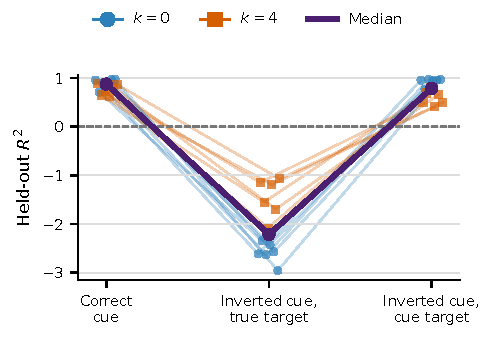
\includegraphics[width=.62\linewidth]{figures/exp2_qwen3_mechanistic_main.pdf}
  \caption{\textbf{Semantic-arm slope decoding follows cue assignment.}
  Each line is a sealed model--$k$ cell across the six open checkpoints of the
  16-episode roster; purple is the median. Probes are fit on correct-context
  development episodes. Under inversion, held-out $R^2$ collapses against the true
  slope and recovers against the cue-assigned slope. The input-embedding control
  below shows this signal is available before any computation, which is why the
  arbitrary-label replication rather than this figure carries the
  representational claim.}
  \label{fig:coin-city-mechanistic-main}
\end{figure}

\begin{figure}[ht]
  \centering
  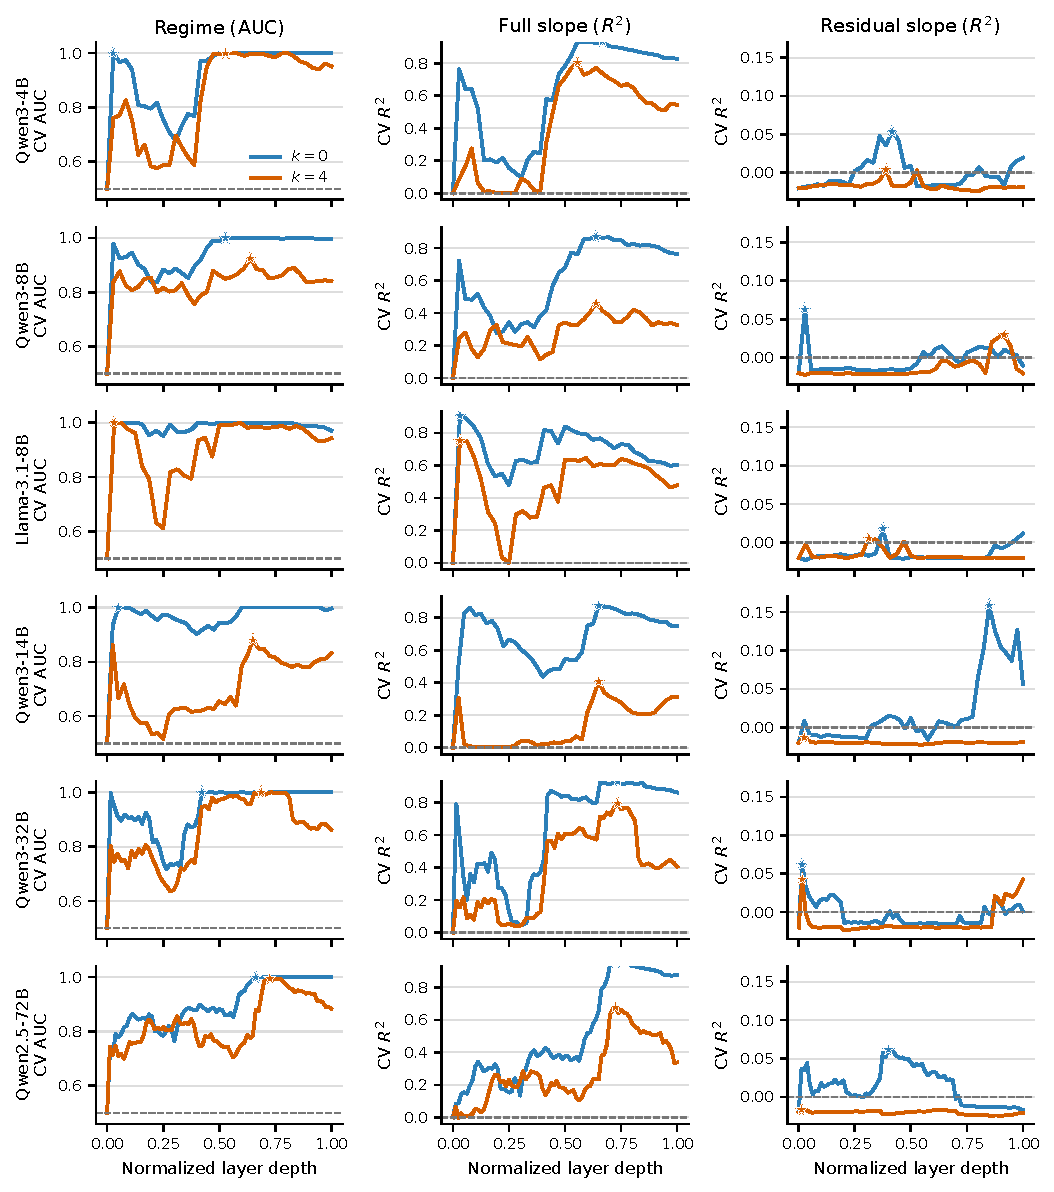
\includegraphics[width=\linewidth]{figures/exp2_qwen3_mechanistic_probe.pdf}
  \caption{\textbf{Development layer trajectories for the six-model probe.}
  Curves show four-fold development CV rather than test performance; stars mark
  the development-selected layer. Layer depth is normalized
  because the checkpoints have 32--80 transformer blocks. The regime and
  full-slope signals are broad, whereas residual-slope CV is weak and does not
  survive held-out evaluation.}
  \label{fig:coin-city-mechanistic-probe}
\end{figure}

\subsubsection{Regime and Full-Slope Decodability}
Across the six checkpoints and two evidence depths, correct-context regime AUC
is $.844$--$1.000$ and full-slope $R^2$ is $.627$--$.975$
(Table~\ref{tab:coin-city-mechanistic-summary}). This information is not a
context-invariant encoding of the true coefficient: removing the City C
description drives selected-layer full-slope $R^2$ below zero in all 12
model--$k$ cells. Under inversion, true-target regime AUC falls to
$.000$--$.109$ while cue-target AUC is $.891$--$1.000$; the full-slope probe
likewise fits the cue-assigned relationship better than the true one. The Llama
replication shows that this pattern is not specific to the Qwen checkpoints.
Across both model families, the linearly available signal therefore tracks the
response family that context assigns to City C.

\subsubsection{What Each Probe Target Can Be Scored Against}
\label{app:coin-city-probe-ceilings}

A probe is scored against a latent generator quantity, so a null is only a fact
about a model if the displayed evidence determines that quantity. We therefore
derive, for each target and evidence depth, the score a Bayes-optimal reader of
the same prompt would obtain. This is an analytic property of
Equation~\ref{eq:coin-city-dgp} and its row construction, computed in closed form
and re-derived by simulating the generator's own row logic; the two agree to
within $.005$ and no model output enters; the derivation is
\path{exp2_v2/biased_news/analysis/compute_bayes_ceilings.py}.
Table~\ref{tab:coin-city-probe-ceilings} gives the ceilings. The same module
reports forecast-MAE floors: $2.28$ poll points at $k=0$ with no cue, $0.17$ for
an oracle told the regime means, and $1.78$ for a reader who must instead estimate
the named regime's slope from its four displayed rows.

The same simulation records one quantity the reference-selection analysis of
Section~\ref{app:coin-city-reference-selection} depends on. Cities draw their
slopes independently, so a reference city's deviation from its regime mean
carries no information about City C's:
$\operatorname{corr}(\widehat\beta^{\mathrm{ref}}-\mu,\;g_C-\mu)=-.0000$ over
400,000 simulated episodes, against a reference-fit standard deviation of $.318$
within regime. That is why a loading on the reference's own sampling error
identifies reference selection, and equally why a forecaster that shrank
optimally would show none.

\begin{center}
\begin{minipage}{\linewidth}
\centering
\captionof{table}{Maximum score a Bayes-optimal reader of the same prompt can
obtain on each probe target, under the frozen data-generating process. The regime
and the full slope are recoverable; the within-regime residual is not, because it
is generated with standard deviation $.03$ while a through-origin fit to City C's
displayed rows carries a standard deviation of $.318$. At $k=0$ City C displays no
rows at all and the residual ceiling is exactly zero.}
\label{tab:coin-city-probe-ceilings}
\small
% Generated by exp2_v2/biased_news/analysis/compute_bayes_ceilings.py; do not edit.
\begin{tabular}{llcc}
\toprule
\textbf{Probe target} & & $k=0$ & $k=4$ \\
\midrule
Regime, correct semantic cue & AUC & 1.000 & 1.000 \\
Regime, arbitrary label & AUC & 0.979 & --- \\
Full slope $g_C$ & $R^2$ & 0.992 & 0.992 \\
Residual slope $g_C-\mu$ & $R^2$ & 0.000 & 0.009 \\
\bottomrule
\end{tabular}

\end{minipage}
\end{center}

\subsubsection{Specificity: Within-Regime Residuals}
The residual target is the specificity control, and it behaves as a target with
no available signal should. The 12 correct-context residual-slope $R^2$ values
range from $-.531$ to $.003$, none of their permutation tests rejects the null
($p=.221$--$.927$), and 33 of 36 arm-level residual scores are nonpositive.
Against a ceiling of $.000$ at $k=0$ and $.009$ at $k=4$, that is the result the
design permits: no reader of these prompts, and no representation computed from
them, could score materially above zero. We therefore read the residual null as
evidence that the probe does not manufacture structure where none is available,
and not as a limit on what these checkpoints encode. A probe that returned a
positive residual score here would be the finding, and it would be a warning
about the probe.

The two recoverable targets do carry information, and the input-embedding control
is what bounds their interpretation. Mean-pooled input embeddings for every Qwen
checkpoint already give perfect regime AUC and full-slope $R^2=.988$--$.993$ under
correct context---at the $.992$ ceiling---because the explicit description names a
regime and the regime means account for essentially all slope variance. Llama
input embeddings likewise give perfect regime AUC and full-slope $R^2=.756/.827$.
The layer-wise semantic result is therefore evidence that the cue-selected
response family is linearly represented, and reaches nothing further about the
continuous $g_C$: the part of $g_C$ beyond the family is not in the prompt to
begin with. The original behavioral inversion screen connects this representation
to output sensitivity in the three larger screened checkpoints: inverted context
raises $k=0$ forecast MAE by $1.66$, $1.96$, and $2.21$ points for 14B, 32B, and
72B, respectively.

\subsubsection{Power-Matched and Cross-Model Arbitrary-Symbol Replication}
\label{app:coin-city-probe-power}

The six-checkpoint roster above seals 16 test episodes per arm. Its exact
label-permutation null spans ROC AUC $[.203,.797]$, so it can separate a score
from chance only above about $.75$. That resolution suffices for the semantic arm,
whose scores sit at ceiling, but it cannot evaluate a weaker signal at all. We
therefore evaluate Qwen3-14B at the design's balanced maximum---248
episodes, 160 development and 88 sealed test, 1,488 activation records---once with
the semantic cue and once with the episode-randomized \texttt{KIV}/\texttt{ZOR}
labels. Anchor, targets, fold structure, ridge grid, layer-selection rule, pooling
controls and the 10,000-repeat held-out permutation test are unchanged; only the
number of episodes differs. The 88-episode null reaches AUC $.603$. The enlarged
development set is disjoint from every episode used by the 16-episode analysis,
providing an independent estimate rather than a re-slice.

\begin{center}
\begin{minipage}{\linewidth}
\centering
\captionof{table}{\textbf{Power-matched Qwen3-14B probe, 88 sealed episodes per
arm.} Correct, none and wrong score the development-selected probe against the true
City C target under the three cue arms; wrong/cue scores the inverted arm against
the relationship its cue names. ``Layer'' is the development-selected block of 40
and ``Embed.'' is the mean-pooled input-embedding control under correct context.
$p$ is the one-sided held-out label-permutation value.}
\label{tab:coin-city-probe-power}
\scriptsize
\setlength{\tabcolsep}{3.2pt}
\resizebox{\linewidth}{!}{% Generated by paper/generate_coin_city_probe_power_table.py; do not edit.
\begin{tabular}{l l rrrr r r r r}
\toprule
Run & Target & Correct & None & Wrong & Wrong/cue & Layer & Embed. & $p$ & Behav. $\Delta\rho$ \\
\midrule
Qwen3-14B, semantic & $k{=}0$ regime AUC & $1.000$ & $.429$ & $.000$ & $1.000$ & 1 & $1.000$ & $<$.001 & --- \\
 & $k{=}4$ regime AUC & $1.000$ & $.560$ & $.000$ & $1.000$ & 1 & $1.000$ & $<$.001 &  \\
 & $k{=}0$ slope $R^2$ & $.942$ & $-.300$ & $-2.806$ & $.961$ & 27 & $.989$ & $<$.001 &  \\
 & $k{=}4$ slope $R^2$ & $.910$ & $-24.039$ & $-2.387$ & $.906$ & 1 & $.989$ & $<$.001 &  \\
\midrule
Qwen3-14B, symbol & $k{=}0$ regime AUC & $.678$ & $.467$ & $.321$ & $.679$ & 26 & $.555$ & $.0016$ & \textbf{$.398$} \\
 & $k{=}4$ regime AUC & $.713$ & $.689$ & $.747$ & $.253$ & 40 & $.582$ & $<$.001 &  \\
 & $k{=}0$ slope $R^2$ & $.016$ & $-.094$ & $-.130$ & $.065$ & 26 & $.003$ & $.1162$ &  \\
 & $k{=}4$ slope $R^2$ & $.030$ & $-.237$ & $.126$ & $-.855$ & 40 & $-.032$ & $<$.001 &  \\
\midrule
Qwen3-8B, symbol & $k{=}0$ regime AUC & $.566$ & $.535$ & $.567$ & $.433$ & 10 & $.534$ & $.1471$ & $.023$ \\
 & $k{=}4$ regime AUC & $.610$ & $.545$ & $.593$ & $.407$ & 19 & $.621$ & $.0401$ &  \\
 & $k{=}0$ slope $R^2$ & $-.001$ & $.005$ & $.004$ & $-.007$ & 25 & $.003$ & $.4883$ &  \\
 & $k{=}4$ slope $R^2$ & $-.151$ & $-.219$ & $-.188$ & $-.504$ & 20 & $-.018$ & $.0314$ &  \\
\midrule
Qwen3-4B, symbol & $k{=}0$ regime AUC & $.520$ & $.419$ & $.329$ & $.671$ & 23 & $.498$ & $.3756$ & $.095$ \\
 & $k{=}4$ regime AUC & $.685$ & $.689$ & $.637$ & $.363$ & 22 & $.585$ & $.0017$ &  \\
 & $k{=}0$ slope $R^2$ & $-.009$ & $-.065$ & $-.079$ & $.023$ & 23 & $.004$ & $.2899$ &  \\
 & $k{=}4$ slope $R^2$ & $-.021$ & $-.265$ & $-.031$ & $-.687$ & 23 & $.004$ & $.0014$ &  \\
\midrule
Qwen2.5-32B, symbol & $k{=}0$ regime AUC & $.778$ & $.571$ & $.200$ & $.800$ & 50 & $.550$ & $<$.001 & \textbf{$.372$} \\
 & $k{=}4$ regime AUC & $.797$ & $.831$ & $.662$ & $.338$ & 46 & $.589$ & $<$.001 &  \\
 & $k{=}0$ slope $R^2$ & $.217$ & $-.256$ & $-1.033$ & $.254$ & 50 & $.004$ & $<$.001 &  \\
 & $k{=}4$ slope $R^2$ & $.263$ & $-.563$ & $-.044$ & $-.774$ & 46 & $-.029$ & $<$.001 &  \\
\midrule
Qwen2.5-72B, symbol & $k{=}0$ regime AUC & $.662$ & $.492$ & $.210$ & $.790$ & 63 & $.556$ & $.0026$ & \textbf{$.381$} \\
 & $k{=}4$ regime AUC & $.793$ & $.745$ & $.651$ & $.349$ & 61 & $.575$ & $<$.001 &  \\
 & $k{=}0$ slope $R^2$ & $-.005$ & $-.490$ & $-1.034$ & $.187$ & 62 & $.004$ & $.0072$ &  \\
 & $k{=}4$ slope $R^2$ & $.222$ & $-.624$ & $-.129$ & $-.870$ & 61 & $-.047$ & $<$.001 &  \\
\midrule
Llama~3.1-8B, symbol & $k{=}0$ regime AUC & $.423$ & $.447$ & $.452$ & $.548$ & 11 & $.539$ & $.8925$ & $.045$ \\
 & $k{=}4$ regime AUC & $.543$ & $.604$ & $.549$ & $.451$ & 31 & $.604$ & $.2470$ &  \\
 & $k{=}0$ slope $R^2$ & $-.097$ & $-.089$ & $-.086$ & $-.001$ & 11 & $.003$ & $.8607$ &  \\
 & $k{=}4$ slope $R^2$ & $-.275$ & $-.091$ & $-.156$ & $-.358$ & 31 & $.009$ & $.4529$ &  \\
\midrule
Llama~3.1-70B, symbol & $k{=}0$ regime AUC & $.728$ & $.468$ & $.292$ & $.708$ & 75 & $.495$ & $<$.001 & \textbf{$.424$} \\
 & $k{=}4$ regime AUC & $.810$ & $.740$ & $.721$ & $.279$ & 42 & $.606$ & $<$.001 &  \\
 & $k{=}0$ slope $R^2$ & $.076$ & $-8.200$ & $-.961$ & $.082$ & 75 & $.003$ & $<$.001 &  \\
 & $k{=}4$ slope $R^2$ & $.222$ & $-3.224$ & $.087$ & $-1.007$ & 55 & $.007$ & $<$.001 &  \\
\bottomrule
\end{tabular}
}
\end{minipage}
\end{center}

The two arms separate sharply, and the input-embedding control is what separates
them. Under the semantic cue the development-selected layer is the first
transformer block for three of the four conditions, and mean-pooled input
embeddings alone already reach regime AUC $1.000$ and full-slope $R^2=.989$: the
decodable quantity is the cue token itself. Under arbitrary labels the same control
collapses to AUC $.555$ and $R^2=.003$, the selected layers move to blocks 26 and
40 of 40, and held-out regime AUC is $.678$ at $k=0$ ($p=.0016$) and $.713$ at
$k=4$ ($p<.001$). The induced label-to-regime mapping is therefore linearly
represented, but only after computation, far more weakly than a regime the model
was told outright, and below the $.979$ AUC a Bayes-optimal reader of the same two
reference cities could reach. Unlike the residual target, the full slope is
recoverable here---its ceiling is $.992$---so its symbol-arm score of $R^2=.016$ at
$k=0$, which does not reject its null, is a genuine gap rather than a property of
the design.

Representation and behavior agree closely once the cue must be induced. On the same
88 sealed episodes the model's own forecasts give regime AUC $.702$, $.518$ and
$.331$ under correct, absent and inverted labels, against probe AUCs of $.678$,
$.467$ and $.321$; inversion raises $k=0$ poll MAE from $2.49$ to $4.28$. With four
City C cases the inverted-arm representation reverses: true-target regime AUC rises
from $.321$ to $.747$, and the full-slope probe fits the cue-named relationship at
$R^2=-.855$ while fitting the true one at $+.126$. Direct target evidence overrides
the induced label in the representation as it does in the forecast.

Six further checkpoints received the identical symbol protocol at the same 88
sealed episodes: Qwen2.5-32B and Qwen2.5-72B, which change model generation;
Qwen3-8B and Qwen3-4B, which hold family, tokenizer and architecture fixed and
change only scale; and Llama~3.1-8B and Llama~3.1-70B, which do the same within a
second vendor and architecture. Held-out regime AUC at $k=0$ is $.778$ for
Qwen2.5-32B ($p<.001$, selected layer 50 of 64), $.728$ for Llama~3.1-70B
($p<.001$, layer 75 of 81), $.662$ for Qwen2.5-72B ($p=.003$, layer 63 of 80),
$.566$ for Qwen3-8B ($p=.15$), $.520$ for Qwen3-4B ($p=.38$) and $.423$ for
Llama~3.1-8B ($p=.89$). No null checkpoint rejects in any $k=0$
condition---regime, slope or residual slope. Mean-pooled input embeddings stay
between $.495$ and $.556$ in every symbol run, so no symbol arm carries the
mapping before computation.

Decodability tracks behavioral recovery across all seven checkpoints, four
positive and three null. The four whose forecasts recover the mapping are the four
in which it decodes (Llama~3.1-70B, $\Delta\rho=.424$; Qwen3-14B, $.398$;
Qwen2.5-72B, $.381$; Qwen2.5-32B, $.372$), and the three whose forecasts do not
are the three in which it does not (Qwen3-4B, $.095$; Llama~3.1-8B, $.045$;
Qwen3-8B, $.023$; all three intervals spanning zero). The Llama~3.1
contrast carries the weight, because it holds family, tokenizer and architecture
fixed, varies only scale, and is the one within-family contrast whose behavioral
classification survives the harder generator population of
Section~\ref{app:coin-city-robustness}: 8B is null on both populations and 70B
positive on both, while the probe runs $.423$ to $.728$ across them. Because the
null and the positive share an architecture and a tokenizer, the split is not an
artifact of either.

The Qwen3 sequence---$.520$, $.566$, $.678$ from 4B to 14B---is consistent with
this but does not add independent weight, because the population that would test
it is the one on which its behavioral boundary moves. That movement is smaller
than the $\Delta\rho$ column alone suggests. Symbol-arm regime accuracy orders the
four Qwen3 checkpoints identically in both populations, $.512$, $.516$, $.660$,
$.656$ originally against $.528$, $.554$, $.589$, $.606$ on the harder one: no
pair reverses, and what changes is that the harder population compresses every
score toward chance, so a threshold that fell in a clear gap now falls inside a
compressed continuum. The $\Delta\rho$ contrast then subtracts a no-context
baseline whose standard error is about $.064$, and baselines of $-.036$ for
Qwen3-8B and $+.025$ for Qwen3-14B are enough to put one interval above zero and
the other $.004$ below it, with the two intervals overlapping by $78\%$. We
therefore read the harder population as showing that the ordering replicates while
the significance threshold is not locatable to a checkpoint, rather than as a
reversal. Section~\ref{app:coin-city-robustness} should be read alongside the
seven-for-seven agreement, which is evidence that the probe reads what the
forecasts express on the episodes both were measured on and not evidence for a
scale law. The positives span three model generations and two
vendors, and every positive shows the same shape: the decoded regime follows the
cue at $k=0$ and the truth at $k=4$.
Qwen3-4B and Qwen3-8B do reject at $k=4$ ($.685$, $p=.002$ and $.610$, $p=.04$),
which is expected rather than contrary: at $k=4$ the displayed target cases
exhibit the regime whatever the label says, and the mean-pooled input embeddings
rise to $.585$ and $.621$ accordingly, in Qwen3-8B's case above the probe itself.
The induction claim is a $k=0$ claim throughout. The sealed test is 88 episodes
per model, well above the 16 the roster began with but not a large sample, and the
permutation nulls are computed rather than assumed.

At 16 episodes, the same arbitrary-symbol procedure returns $k=0$ regime AUC
$.312$ with $p=.90$. Its $[.203,.797]$ null is too broad to resolve a signal of
the magnitude observed at 88 episodes.

\subsubsection{Causal Test: Patching the City C Label Representation}
\label{app:coin-city-causal-patch}

Decodability is not mediation. To test whether the representation the probe reads
is the one the forecast uses, we intervene on it directly. Under arbitrary labels, an episode's correct and swapped prompts are
positionally aligned through the City C label and differ at exactly two label-token
positions.
We replace the residual stream at those two positions with the states the opposite
arm produces, in both directions, and regenerate the forecast greedily. The
endpoint is the episode-level mean of the regime-aligned correct-into-swapped
shift and the sign-reversed swapped-into-correct shift, tested one-sided against
an episode sign-flip null.

The analysis uses three patch sites and two controls. The primary site is a
three-layer window centred on the development-selected relational layer;
patching at the embedding output only, and at every causally effective layer, are
the comparison sites; the unpatched arm and a self-patch that writes each state
back over itself are the controls. Layer, window and ridge were selected on
development episodes with the sealed test unread.

\begin{center}
\begin{minipage}{\linewidth}
\centering
\captionof{table}{\textbf{Causal effect of patching the two City C symbol
subtokens, Qwen3-14B.} Shift is the regime-aligned symmetric patch mean; positive
means the forecast moved toward the relationship the donor label names. The
16- and 88-episode analyses select their windows independently on
their own development sets. The null interval is the 88-episode sign-flip null.}
\label{tab:coin-city-causal-patch}
\small
\setlength{\tabcolsep}{4pt}
\resizebox{\linewidth}{!}{% Generated by paper/generate_coin_city_causal_patch_table.py; do not edit.
\begin{tabular}{l c rrr rrr c}
\toprule
& & \multicolumn{3}{c}{16 sealed, window 33--35} & \multicolumn{3}{c}{88 sealed, window 19--21} & \\
\cmidrule(lr){3-5}\cmidrule(lr){6-8}
Patch site & $k$ & Shift & $p$ & $n$ & Shift & $p$ & $n$ & Null 95\% \\
\midrule
Selected window & $k{=}0$ & $-.033$ & $.75$ & 14 & $.333$ & $<$.0001 & 82 & $[-.177,.178]$ \\
 & $k{=}4$ & $-.007$ & $.75$ & 15 & $-.035$ & $.8256$ & 87 & $[-.073,.073]$ \\
\midrule
Embedding only & $k{=}0$ & $.236$ & $.15$ & 14 & $.319$ & $.0002$ & 84 & $[-.182,.182]$ \\
 & $k{=}4$ & $.115$ & $.23$ & 15 & $-.017$ & $.6419$ & 87 & $[-.087,.087]$ \\
\midrule
All layers & $k{=}0$ & $.236$ & $.15$ & 14 & $.319$ & $.0002$ & 84 & $[-.182,.182]$ \\
 & $k{=}4$ & $.115$ & $.23$ & 15 & $-.017$ & $.6419$ & 87 & $[-.087,.087]$ \\
\bottomrule
\end{tabular}
}
\end{minipage}
\end{center}

At $k=0$ the intervention moves the forecast: patching the selected window shifts
the regime-aligned prediction by $.333$ against a null interval of
$[-.177,.178]$ ($p<.0001$, 82 complete episodes), and patching the embedding
alone gives $.319$. All eight stability checks pass, including $347/347$ exact
self-patch matches.

Two readings of the table matter more than the significance. First, the
embedding-only and all-layer rows are identical, and necessarily so: the two
prefixes differ only at the patched label positions, so overwriting their embeddings
and letting the model recompute reproduces what overwriting every later state does. They are one intervention reported at two depths, not two
converging results. What distinguishes the mid-window row is that it reaches the
same magnitude while touching only three layers late in the network.

Second, the effect is confined to $k=0$. With four City C cases every patch site
returns a null ($p=.83$ and $p=.64$), so the induced label no longer controls the
forecast once direct target evidence is available. That is the revision claim of
Section~\ref{app:coin-city-results} in causal form, and it matches the
representational result: at $k=4$ the inverted-arm probe recovers the true regime
rather than the cue-assigned one.

At 16 episodes, the primary patch estimate is $-.033$ at $p=.75$ and the sign-flip
null spans $[-.387,.387]$. Its 64-episode development set selects layers
$33$--$35$, whereas the 160-episode development set selects $19$--$21$ at a
higher cross-validation score ($.903$ against $.806$).

\paragraph{Permutation implementation.} The test enumerates all $2^{n}$ sign
assignments for 16 episodes; exhaustive enumeration is infeasible for 88
($2^{88}\approx3\times10^{26}$). Enumeration is retained for $n\le20$; above it
the same null is sampled with $200{,}000$ draws under a fixed seed, giving a
Monte Carlo standard error of $.0005$ at $p=.05$. The estimand, endpoint, and
direction are identical under both implementations.

\paragraph{Scope.} This is one checkpoint under arbitrary labels. It shows that
the label representation Qwen3-14B computes is causally responsible for its
zero-shot regime assignment, and that direct evidence displaces it. It does not
establish the same for the hosted deployments, the semantic cue, or other
architectures.

\subsubsection{Reproducibility and Scope}
The checkpoints are pinned to commits
\texttt{cdbee75f17c01a7cc42f958dc650907174af0554} (Qwen3-4B),
\texttt{b968826d9c46dd6066d109eabc6255188de91218} (Qwen3-8B),
\texttt{0e9e39f249a16976918f6564b8830bc894c89659} (Llama-3.1-8B),
\texttt{40c069824f4251a91eefaf281ebe4c544efd3e18} (Qwen3-14B),
\texttt{9216db5781bf21249d130ec9da846c4624c16137} (Qwen3-32B), and
\texttt{495f39366efef23836d0cfae4fbe635880d2be31} (Qwen2.5-72B).
The activation hashes are
\texttt{e1913859\allowbreak{}63d639aa\allowbreak{}5b8574a9\allowbreak{}abbeb91b\allowbreak{}3519aed9\allowbreak{}34ac491f\allowbreak{}86365563\allowbreak{}1b26dbbc}
(Qwen3-4B) and
\texttt{7f65aeec\allowbreak{}7a91e404\allowbreak{}cc600686\allowbreak{}18fedf25\allowbreak{}c679abde\allowbreak{}5d48c2b8\allowbreak{}477f7366\allowbreak{}70fbc54f}
(Llama-3.1-8B); all six hashes and tensor dimensions are enforced by the
fail-closed generator. Frozen tasks, activation tensors, extraction manifests,
generated behavior, selected predictions, complete layer curves, and probe
results are under
\path{exp2_v2/biased_news/data/coin_city_stable_relationship_claude_n250_v4/mechanistic_probe/}.
The analysis and asset generator are
\path{exp2_v2/biased_news/mechanistic_probe/analyze_probe.py} and
\path{paper/generate_coin_city_mechanistic_comparison.py}. The causal run is
\path{mechanistic_probe/qwen3_14b_symbol_relational_v2/}, frozen by
\path{freeze_symbol_relational_protocol.py} and executed by
\path{extract_symbol_label_states.py}, \path{patch_symbol_label_activations.py}
and \path{analyze_symbol_relational_probe.py}; every count in that pipeline is
derived from the frozen task manifest and checked by
\path{tests/test_symbol_relational_scaling.py}.
\path{paper/generate_coin_city_causal_patch_table.py} fails closed on the run's
study name, sealed-test size and stability gate. The power-matched runs are
\path{mechanistic_probe/qwen3_14b_probe_v2/},
\path{mechanistic_probe/qwen3_14b_symbol_probe_v2/},
\path{mechanistic_probe/qwen3_8b_symbol_probe_v2/},
\path{mechanistic_probe/qwen3_4b_symbol_probe_v2/},
\path{mechanistic_probe/llama3_1_70b_symbol_probe_v2/},
\path{mechanistic_probe/qwen2_5_72b_symbol_probe_v2/},
\path{mechanistic_probe/qwen2_5_32b_symbol_probe_v2/} (checkpoint
\texttt{5ede1c97bbab6ce5cda5812749b4c0bdf79b18dd}) and
\path{mechanistic_probe/llama3_1_8b_symbol_probe_v2/} (checkpoint
\texttt{0e9e39f249a16976918f6564b8830bc894c89659}), built by
\path{exp2_v2/biased_news/mechanistic_probe/build_probe_tasks.py} and
\path{build_arbitrary_symbol_probe_tasks.py} with 62 and 31 episodes per factorial
cell; \path{paper/generate_coin_city_probe_power_table.py} regenerates their table
and validates the sealed-test size and task hash. Each run's
activation tensor is regenerable from its frozen task file and pinned checkpoint;
the extraction manifests record the tensor hashes rather than the tensors.
Cross-vendor probe evidence here is the Llama~3.1-8B null rather than a
positive. The diagnostic covers six checkpoints spanning Qwen and Llama at 16 sealed episodes per arm, plus
the matched 88-episode semantic and arbitrary-symbol Qwen3-14B pair. For the semantic
cue it is correlational and does not establish that the decoded direction
mediates the forecast; under arbitrary labels
Section~\ref{app:coin-city-causal-patch} provides a causal intervention for one
checkpoint. Both complement the paired behavioral interventions above.
